\section{Measurement Model}
\label{sec:measurement_model}

As explained in Sect.~\ref{section:explorative_information_cost_function}, each future position $x_{j}$ will generate a multi-beam range measurement $z_{j}$. We express each measurement as a $K$-tuple random variable, $z_{j} = \left[z_{j, 1}, \dots, z_{j, K}\right]$, with $z_{j, k} \in \left[z_{min}, z_{max}\right]$. A measurement model is required to sample from the distribution $p(z_{\tau})$. Assuming laser beam independence, $p(z_{\tau})$ can be expressed as a product of the measurement probabilities of individual beams at each timestep over the interval $\tau = t+1:t+T$.
%
\begin{align}
  \begin{split}
    p
    \left(
    z_{\tau}
    \right)
    &=
    \prod_{j=t+1}^{t+T}
    \prod_{k=1}^{K}
    p
    \left(
    z_{j, k}
    \right)
  \end{split}
\end{align}
%
The probability of a single beam measurement can be expressed as a function of the true distance, $r$, to the obstacle.
%
\begin{align}
  \begin{split}
    p
    \left(
    z_{j, k}
    \right)
    &=
    \int_{r}
    p
    \left(
    z_{j, k}
    \ \vert \
    r
    \right)
    p
    \left(
    r
    \right)
    dr
  \end{split}
\end{align}
%
\begin{align}
  \begin{split}
    p
    \left(
    z_{j, k}
    \ \vert \
    r
    \right)
    &=
    \left\{
    \begin{array}{ll}
      \mc{N}(z_{j, k} - r, \sigma_{hit}^{2}) &: z_{min} \le r \le z_{max} \\
            \mc{N}(z_{max}, \sigma_{hit}^{2}) &: z_{max} < r \\
                                            0 &: r < z_{min}
    \end{array}
    \right.
    \label{eq:measurement_model}
  \end{split}
\end{align}
%
where $\mc{N}(x - \mu, \sigma^{2})$ is a one-dimensional Gaussian with mean $\mu$ and variance $\sigma^{2}$. The Gaussian term in Eq.~\eqref{eq:measurement_model} is an approximation for the true distribution, which is a complex function of both beam angle as well as non-axial distance-dependent noise. The environment-dependent distribution $p(r)$ corresponds to the probability that an obstacle intersects a beam at range $r$. We model this as a Poisson binomial distribution with probabilities decaying according to the inverse square of the beam range.

On the interval $\left[z_{min}, z_{\max}\right]$, $p(z_{j, k})$ reduces to a Gaussian convolution with $p(r)$ over $r$, which can be computed in $O(n \log n)$ operations with a Fast Fourier Transform. This computation can be reduced to $O(n)$ by assuming that $\sigma_{hit}$ of the range sensor is much smaller than the resolution of the map.

The distribution $p(r)$ represents the probability that the first obstacle along a ray originating at the sensor is found at distance $r$. $p(r)$ can be expressed as a generalization of the geometric distribution for independent, but not identically distributed (i.n.i.d.) Bernoulli trials.
%
\begin{align}
  \begin{split}
    p(r = i)
    &=
    p_{t}(m^i)
    \prod_{j=1}^{i-1}
    \left(
      1 - p_{t}(m^{j})
    \right)
    \\
    &=
    p_{t}(m^i)
    \left(
      \frac{1}{p_{t}(m^{i-1})} - 1
    \right)
    p(r = i - 1)
  \end{split}
\end{align}


\begin{figure}
  \centering
  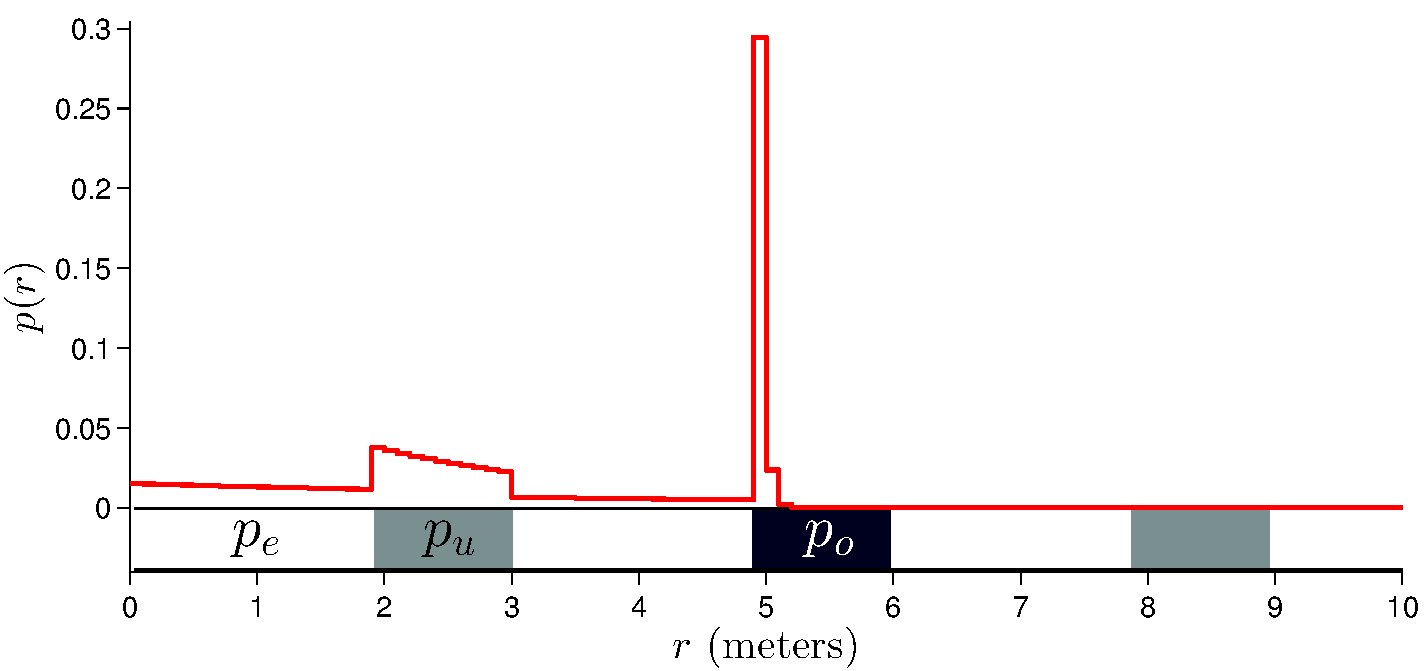
\includegraphics[width=1.0\textwidth]{meas_model.pdf}
  \caption{The distribution $p(r \ \vert \ m)$ over a depicted 1-dimensional map with resolution $\Delta r = 0.1$ m, and $p_{e} = 0.01$, $p_{o} = 0.92$, $p_{u} = 0.05$. \label{fig:measurement_model}}
\end{figure}

